\chapter{Anexos Técnicos}

Los anexos reúnen información de soporte que complementa el cuerpo del estudio: el diagrama unifilar del circuito, el esquema de componentes del proyecto, el perfil horario completo de demanda, especificaciones resumidas, la matriz de impacto, el cronograma de validación sugerido y las referencias documentales.

\section{Diagrama Unifilar del Circuito 10-502}

La Figura~\ref{fig:unifilar} reproduce el diagrama unifilar del circuito 10-502 entregado por ESSA. Este plano constituye la referencia topológica del modelo eléctrico empleado en los análisis de flujo de carga, cortocircuito y protecciones.

\begin{figure}[p]
    \centering
    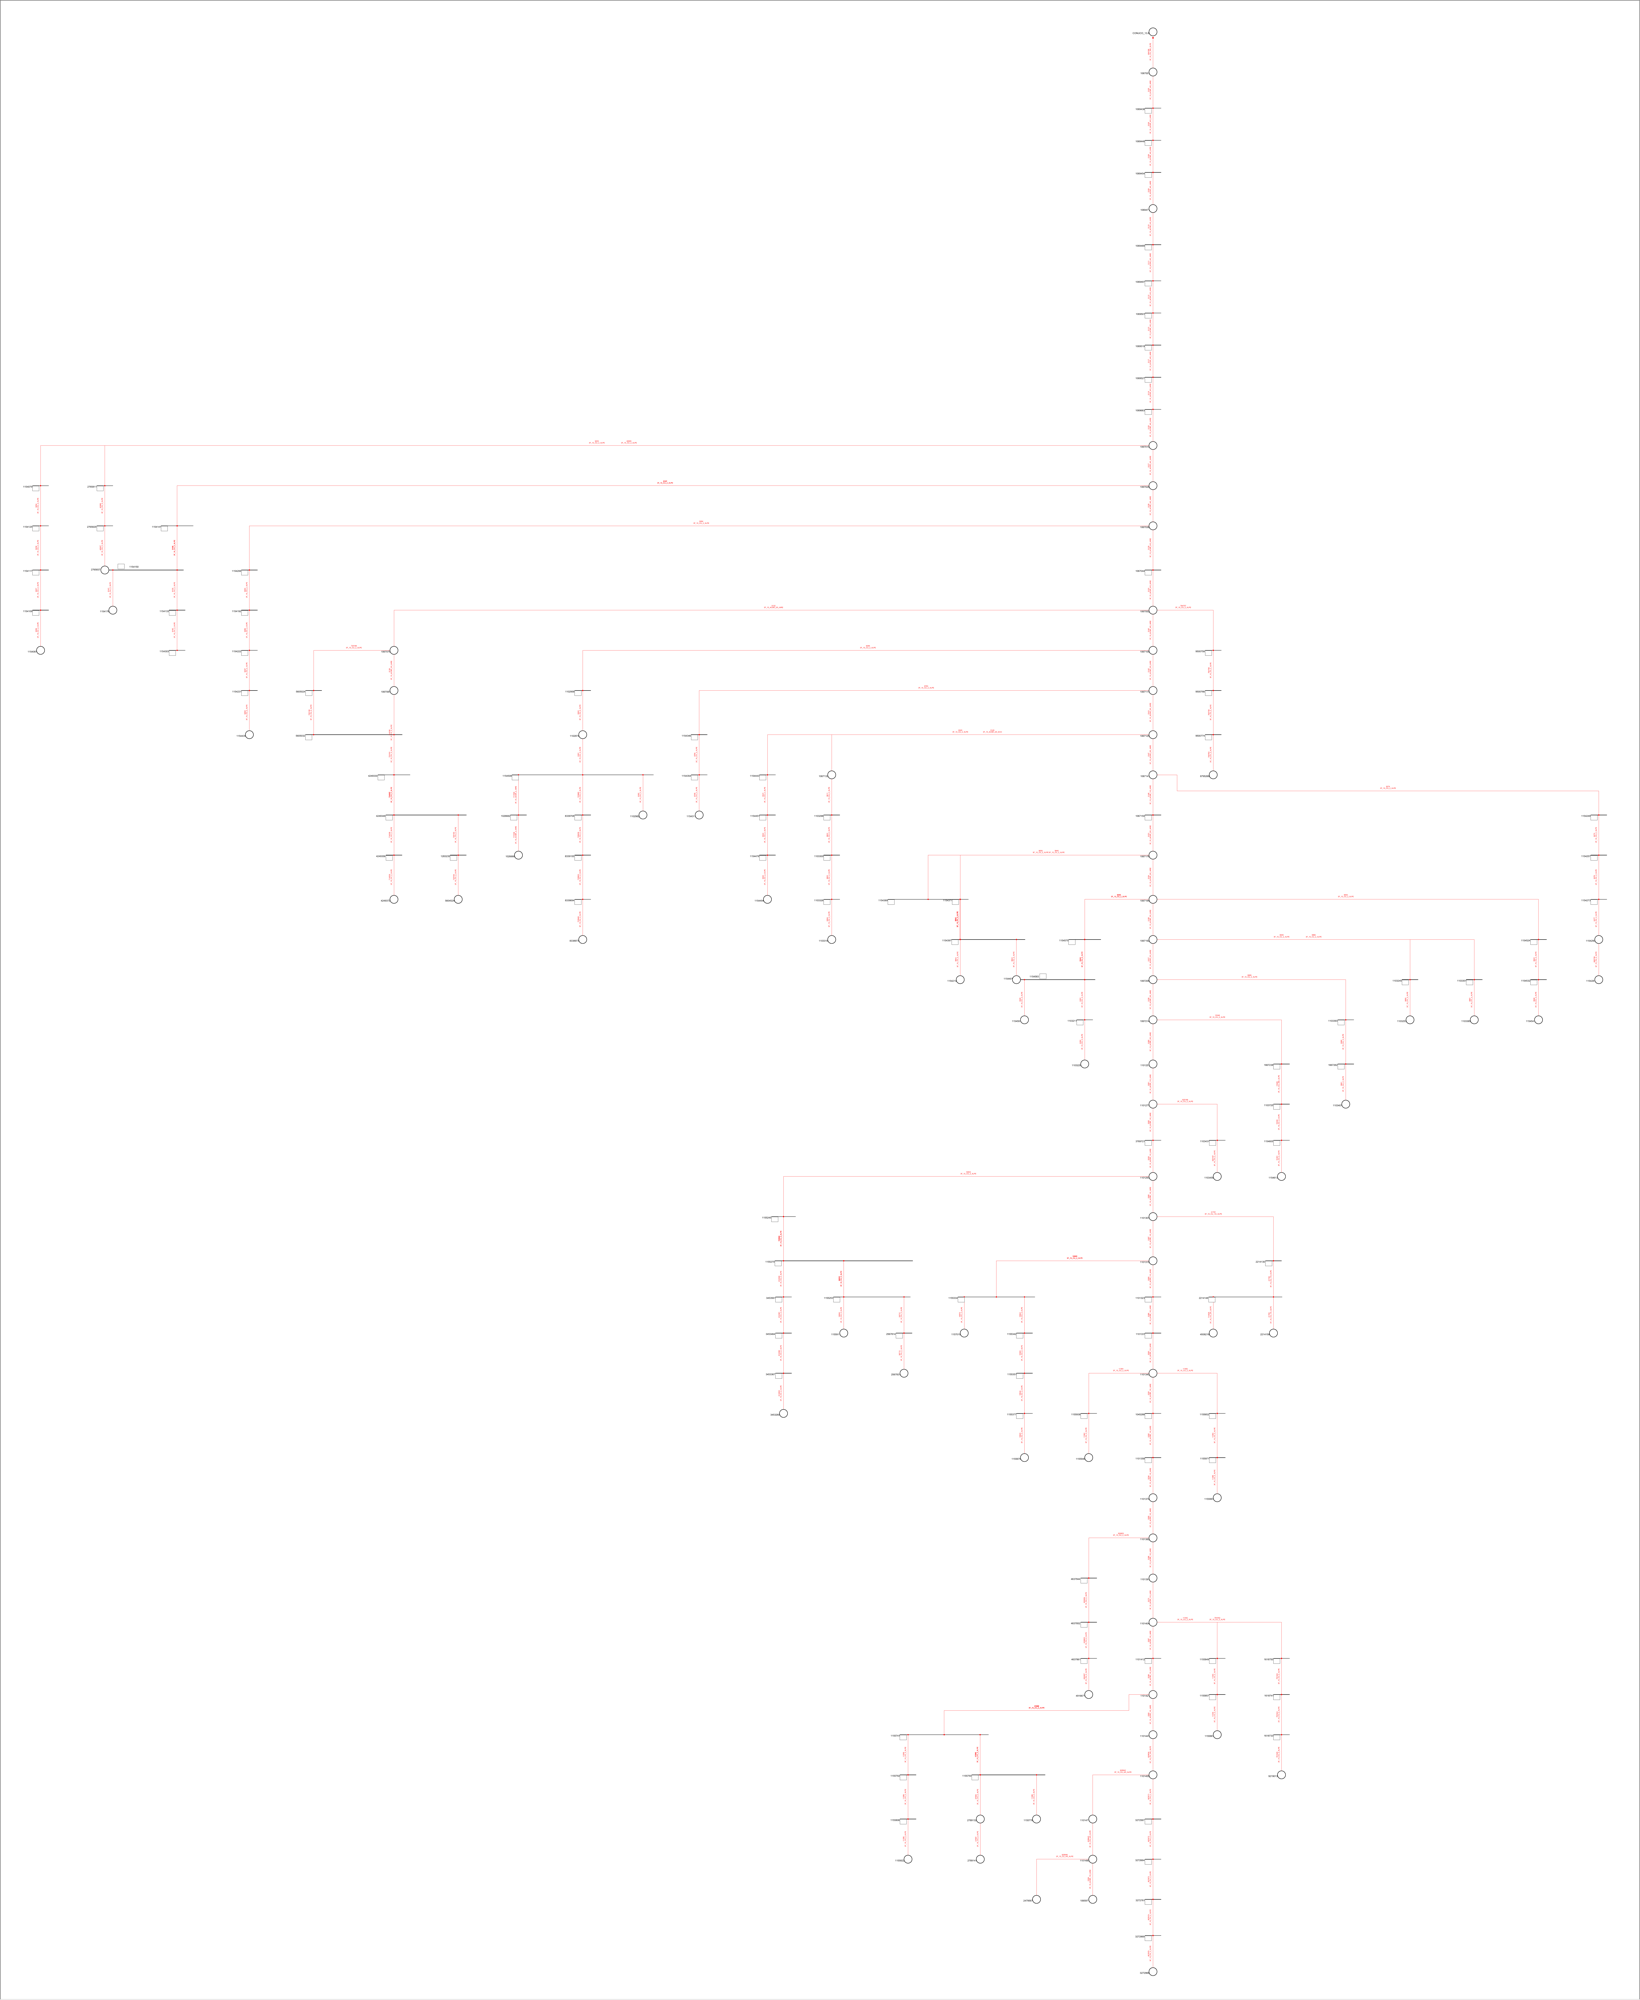
\includegraphics[width=\textwidth,height=0.72\textheight,keepaspectratio]{figuras/cto_10502-1.png}
    \caption{Diagrama unifilar del circuito 10-502 (fuente: ESSA)}
    \label{fig:unifilar}
\end{figure}
\clearpage

\section{Esquema de Componentes del Proyecto}

La cadena de componentes del sistema fotovoltaico, desde el campo solar hasta la red de ESSA, se resume a continuación. El arreglo de 240 paneles de 590~W (141,6~kWp) alimenta dos inversores SOLIS de 60~kW (120~kW~AC); la protección de inversor y de acometida se sitúa aguas arriba del transformador de 150~kVA (13,2~kV/220~V, Dyn5), el cual se conecta al nodo 3272966 del circuito 10-502 a 13,8~kV.

\begin{center}
    \begin{tabular}{c}
    \toprule
    \textbf{COMPONENTES DEL SISTEMA} \\
    \midrule
    \\
    Paneles Fotovoltaicos \\
    (240 $\times$ 590 W = 141,6 kWp) \\
    \textbar \\
    Inversores SOLIS \\
    (2 $\times$ 60 kW = 120 kW AC) \\
    \textbar \\
    Protección de Inversor \\
    (3 $\times$ 140--200 A) \\
    \textbar \\
    Protección de Acometida \\
    (3 $\times$ 350--500 A) \\
    \textbar \\
    Transformador de Conexión \\
    (150 kVA, 13,2 kV/220 V, Dyn5) \\
    \textbar \\
    Red de ESSA --- Circuito 10-502 \\
    (Nodo 3272966, 13,8 kV) \\
    \\
    \bottomrule
    \end{tabular}
\end{center}

\section{Perfil Horario Completo de Demanda}

La Tabla~\ref{tab:demanda_24h} presenta el registro completo de demanda en cabecera del circuito 10-502 para el día 19/03/2024, base del ajuste horario utilizado en el flujo de carga. El perfil confirma el valle nocturno, la rampa matutina y el pico cercano al mediodía descritos en el cuerpo del estudio.

\begin{table}[H]
    \centering
    \small
    \caption{Demanda en cabecera del circuito 10-502 (19/03/2024)}
    \label{tab:demanda_24h}
    \begin{tabular}{ccc}
    \toprule
    \textbf{Hora} & \textbf{I [A]} & \textbf{S [MVA]} \\
    \midrule
    00:00 & 34,99 & 0,836 \\
    01:00 & 33,26 & 0,795 \\
    02:00 & 31,86 & 0,762 \\
    03:00 & 28,46 & 0,680 \\
    04:00 & 26,35 & 0,630 \\
    05:00 & 26,78 & 0,640 \\
    06:00 & 29,72 & 0,710 \\
    07:00 & 35,62 & 0,851 \\
    08:00 & 50,59 & 1,209 \\
    09:00 & 61,05 & 1,459 \\
    10:00 & 66,21 & 1,583 \\
    11:00 & 69,70 & 1,666 \\
    12:00 & 70,41 & 1,683 \\
    13:00 & 67,38 & 1,611 \\
    14:00 & 64,58 & 1,544 \\
    15:00 & 68,55 & 1,638 \\
    16:00 & 68,78 & 1,644 \\
    17:00 & 67,10 & 1,604 \\
    18:00 & 62,31 & 1,489 \\
    19:00 & 55,36 & 1,323 \\
    20:00 & 49,48 & 1,183 \\
    21:00 & 44,82 & 1,071 \\
    22:00 & 40,30 & 0,963 \\
    23:00 & 37,40 & 0,894 \\
    \bottomrule
    \end{tabular}
\end{table}

\section{Especificaciones Técnicas Resumen}

La Tabla~\ref{tab:espec_resumen} concentra las especificaciones técnicas generales del proyecto, desde la ubicación geográfica hasta el circuito y el nodo de conexión. Sirve como ficha de referencia rápida para revisiones posteriores o para la elaboración de memorias de cálculo complementarias.

\begin{table}[H]
    \centering
    \caption{Especificaciones técnicas generales del proyecto}
    \label{tab:espec_resumen}
    \begin{tabular}{ll}
    \toprule
    \textbf{Parámetro} & \textbf{Valor} \\
    \midrule
    Ubicación & Bucaramanga, Santander \\
    Latitud / Longitud & 7,12621563° / $-$73,11227598° \\
    Capacidad instalada DC / AC & 141,6 kWp / 120 kW \\
    Tecnología & Paneles monocristalinos JINKO \\
    Número de paneles / potencia & 240 / 590 W \\
    Eficiencia de paneles & 22,84\% \\
    Inversores & 2 $\times$ SOLIS 60K-LV-5G \\
    Factor de potencia & 0,99 \\
    Tensión de salida & 220 VAC, 60 Hz \\
    Relación DC/AC & 1,18 \\
    Transformador & 150 kVA, 13,2/0,22 kV, Dyn5 \\
    Circuito / POC & 10-502 / Nodo 3272966 \\
    Nivel de tensión conexión & 13,8 kV \\
    Año de entrada en operación & 2025 \\
    \bottomrule
    \end{tabular}
\end{table}

\section{Matriz de Evaluación de Impacto}

La matriz de la Tabla~\ref{tab:matriz_impacto} sintetiza el cumplimiento de los parámetros críticos del sistema frente a sus límites operativos. En todos los casos el proyecto cumple, con impactos mínimos o positivos sobre tensión, cargabilidad, cortocircuito, factor de potencia y pérdidas técnicas.

\begin{table}[H]
    \centering
    \caption{Evaluación de impacto en parámetros del sistema}
    \label{tab:matriz_impacto}
    \begin{tabular}{lcccc}
    \toprule
    \textbf{Parámetro} & \textbf{Límite} & \textbf{Máximo} & \textbf{Cumple} & \textbf{Impacto} \\
    \midrule
    Tensión (p.u.) & 0,90--1,10 & 0,9953 & $\checkmark$ & Mínimo \\
    Cargabilidad líneas (\%) & $\leq$ 100 & 4,57 & $\checkmark$ & Mínimo \\
    Cargabilidad trafo (\%) & $\leq$ 100 & 55,83 & $\checkmark$ & Bajo \\
    Variación CC & $<$ 1\% & $\approx$0\% & $\checkmark$ & Nulo \\
    Factor de potencia & $\geq$ 0,90 & 0,99 & $\checkmark$ & Positivo \\
    Pérdidas técnicas (kW) & Reducción & $-$0,34 & $\checkmark$ & Positivo \\
    \bottomrule
    \end{tabular}
\end{table}

\section{Cronograma de Validación Recomendado}

Para acompañar la puesta en servicio se propone el cronograma de la Tabla~\ref{tab:cronograma}, que cubre inspección y pruebas de protecciones en pre-operación, mediciones de calidad durante el primer mes, validación de tensiones a tres meses y reportes periódicos de desempeño. La responsabilidad compartida entre COPOWER y ESSA garantiza trazabilidad técnica ante el operador.

\begin{table}[H]
    \centering
    \caption{Actividades de validación post-conexión}
    \label{tab:cronograma}
    \begin{tabular}{llcl}
    \toprule
    \textbf{Fase} & \textbf{Actividad} & \textbf{Plazo} & \textbf{Responsable} \\
    \midrule
    Pre-operación & Inspección de instalaciones & 2 semanas & COPOWER + ESSA \\
    Pre-operación & Pruebas de protecciones & 2 semanas & COPOWER + ESSA \\
    Operación & Mediciones de calidad & 1 mes & COPOWER + ESSA \\
    Operación & Validación de tensiones & 3 meses & ESSA \\
    Operación & Reporte de desempeño & Trimestral & COPOWER \\
    \bottomrule
    \end{tabular}
\end{table}

\section{Documentos de Referencia}

El estudio se apoya en el siguiente cuerpo normativo y documental: Resoluciones CREG~030 de 2018 (conexión de generadores), CREG~025 de 1995 (Código de Redes) y CREG~174 de 2021 (autogeneración a pequeña escala); Acuerdo~1322 del CNO sobre protecciones de generadores; normas IEC~60909 e IEEE~242; los archivos \textit{Datos Circuito 10 502 - 2026.xlsx} y \textit{CTO 10 502.pdf} entregados por ESSA; y las fichas técnicas del inversor SOLIS~60K-LV-5G y de los paneles JINKO monocristalinos.

\section{Contacto}

\begin{center}
    \textbf{COPOWER LTDA} \\
    Especialistas en Energías Renovables \\
    Bucaramanga, Santander --- Colombia \\
    Julio de 2026
\end{center}
